% -*- mode:LaTeX; mode:flyspell; mode:hl-line; -*-
\documentclass{article}

% Almost always
\usepackage{enumerate}
\usepackage{booktabs}
\usepackage{amsmath, amsthm}
\usepackage{graphicx}
\usepackage{color}
\usepackage[verbose,letterpaper,top=1.25in,bottom=1in,left=1.25in,right=1.25in]{geometry}

\setlength{\parindent}{0pt}
\setlength{\parskip}{\baselineskip}

% extra stuff for assignments
\newcounter{totalpoints}
\setcounter{totalpoints}{0}

\newcommand{\points}[1]{{\addtocounter{totalpoints}{#1}\textbf{[#1 points]}}}
\usepackage{environ}
\usepackage{etoolbox}
\makeatletter
\NewEnviron{answer}[1]
{\ifx\BODY\@empty
 \vspace{#1}%
\else
{\par\sf\color{blue} \BODY}%
\fi}
\makeatother

\usepackage{totcount}
\regtotcounter{totalpoints}
\begin{document}

{\bigskip\hrule\bigskip
\huge
\noindent CMPUT 366, Winter 2022\\
Assignment \#2

\large
Due: Monday, Feb.\ 28, 2022, 11:59pm\\
Total points: \total{totalpoints}

For this assignment use the following consultation model:
\begin{enumerate}

\item you can discuss assignment questions and exchange ideas with other \emph{current} CMPUT~366 students;

\item you must list all members of the discussion in your solution;

\item you may {\bf not} share/exchange/discuss written material and/or code;

\item you must write up your solutions individually;

\item you must fully understand and be able to explain your solution in any amount of detail as requested by the instructor and/or the TAs.

\end{enumerate}

Anything that you use in your work and that is not your own creation must be properly cited by listing the original source. Failing to cite others' work is plagiarism and will be dealt with as an academic offense.

%%%%%%%%%%%%%%%%%%%%%%%%%%%%%%%%%%%%%

\bigskip\bigskip\hrule\bigskip

\vspace{1cm}
\hspace{1cm}{\bf First name:} \underline{\hspace{7cm}}

\vspace{1cm}
\hspace{1cm}{\bf Last name:} \underline{\hspace{7cm}}

\vspace{1cm}
\hspace{1cm}{\bf CCID:} \underline{\hspace{5.5cm}}\verb|@ualberta.ca|

\vspace{1cm}
\hspace{1cm}{\bf Collaborators:} \underline{\hspace{6.5cm}}

\vspace{1cm}
\bigskip\hrule\bigskip
}

\pagestyle{myheadings}
\markboth{}{CMPUT 366 --- Assignment \#2}

%% Comments for next time
% - don't ask them to prove something is NOT identifiable, that's nuts, just ask if it satisfies the back-door criterion (or ask about something that IS identifiable, by the back-door criterion).
% - be clear in the efficiency question that all the variables have the same size of domain.
% - Variable elimination query should be P(B|G=true,E=true)

These are example solutions for assignment 2.

\begin{enumerate}

%------------------------------------------------------------------------------------------
\item \textbf{(Probability theory)}

\begin{enumerate}
\item \points{20}

Consider the following scenario.
2\% of the people who walk through a specific metal detector at YEG are carrying a gun.
30\% of the people who walk through the same metal detector are carrying coins.
The remaining 68\% are carrying nothing made of metal.
Everyone carries either nothing, coins, or a gun through the detector; never both coins and a gun.

If someone carries a gun through this metal detector, it will beep with probability 95\%.
If someone carries coins through this same metal detector, it will beep with probability 80\%.
If someone carries nothing made of metal through the detector, it will still beep about 25\% of the time.

Suppose that the metal detector beeps when someone walks through it.  With what probability is that person carrying a gun?  Show how you calculated your answer.

\begin{answer}{1.5in}
% put your answer here
\end{answer}

\end{enumerate}

\clearpage
%------------------------------------------------------------------------------------------
\item (\textbf{Belief networks})

\begin{enumerate}
\item \points{5}
What factorization of the joint distribution $P(A,B,C,D,E,F,G)$ does the network below represent?

\begin{center}
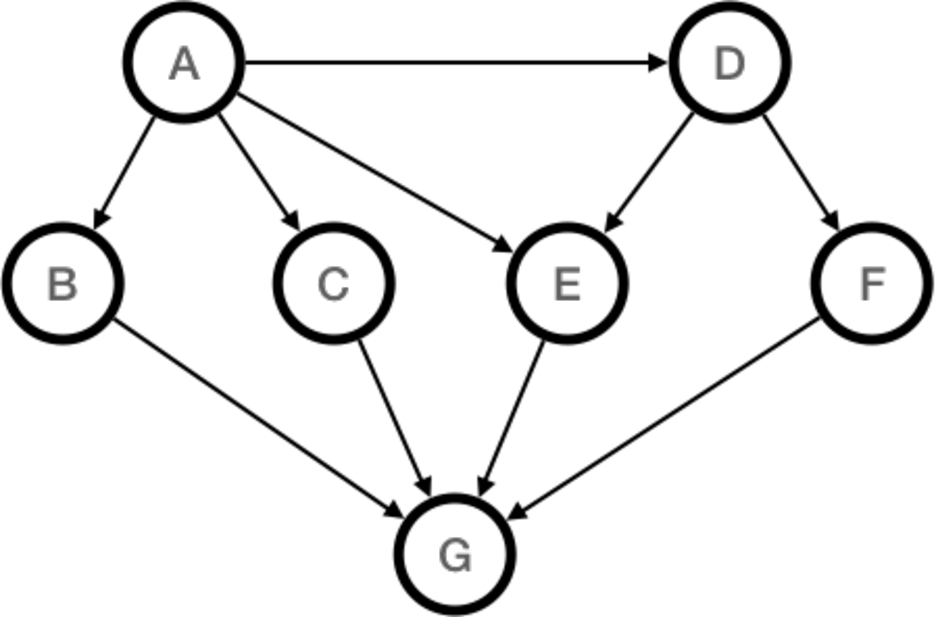
\includegraphics[width=.25\textwidth]{a2-q2a.pdf}    
\end{center}

\begin{answer}{.5in}
% put your answer here
\end{answer}

\item \points{5} \label{q:joint}
Draw a belief network that is consistent with a joint distribution that factors as
$P(A,B,C,D,E) = P(E| C,D)P(D | C)P(C | A,B)P(B | A)P(A)$.

For \textbf{5 bonus marks}, draw another, different belief network that is \emph{also} consistent with this factoring.

\begin{answer}{2in}
% put your answer here
\end{answer}

\item \points{3}
Suppose that every random variable in the joint distribution of question~(\ref{q:joint}) has a domain containing $10$ elements.  How many rows are needed to list the full joint distribution in an explicit table?

\begin{answer}{.5in}
% put your answer here
\end{answer}

\item \points{7}
Suppose that every random variable in the joint distribution of question~(\ref{q:joint}) has a domain containing $10$ elements.  How many rows in total are needed to list the conditional probability tables for your belief network representation?

\begin{answer}{.5in}
% put your answer here
\end{answer}
\end{enumerate}

\clearpage
%------------------------------------------------------------------------------------------
\item \textbf{(Variable Elimination)}
Consider the belief network below.

\begin{center}
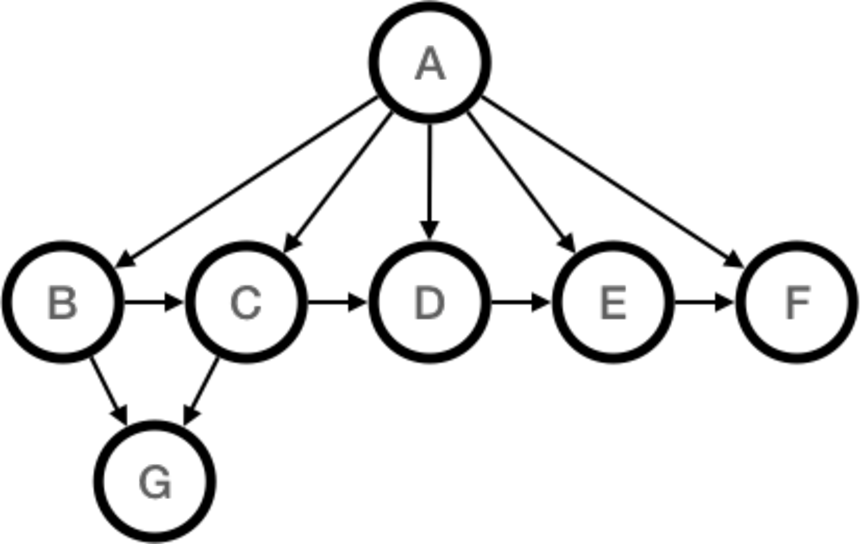
\includegraphics[width=.25\textwidth]{a2-q3.pdf}    
\end{center}

\begin{enumerate}
    \item \points{15}
    List the factors that would be created, and the operations used to create them, by running the variable elimination algorithm on this belief network to answer the query $P(B|G,E)$.
    Use the variable ordering $G,E,A,B,C,D,F$.



    \begin{answer}{1.5in} \label{q:order-a}
    % put your answer here
    \end{answer}

    \item \points{15} \label{q:order-b}
    List the factors that would be created, and the operations used to create them, by running the variable elimination algorithm on this belief network to answer the query $P(B|G,E)$.
    Use the variable ordering $G,E,F,D,C,B,A$

    \begin{answer}{1.5in}
    % put your answer here
    \end{answer}

    \item \points{5}
    Which of the two given variable orderings is more efficient for this query?  Justify your answer.
    You may assume that the domain of each variable is the same size.

    \begin{answer}{.5in}
    % put your answer here
    \end{answer}

\end{enumerate}

\newcommand{\Books}{B}
\newcommand{\Read}{R}
\newcommand{\Like}{L}
\newcommand{\Tests}{T}

\clearpage
%------------------------------------------------------------------------------------------
\item \textbf{(Causal inference)}

Consider the following causal model containing random variables \{\Like, \Read, \Books, \Tests\}, with $\text{dom}(\Tests)=\{high,low\}$, $\text{dom}(\Books)=\{many,few\}$,
and all other variables having domain $\{true,false\}$.  

The variable $\Like$ indicates that the parents in a house {like to read}.
The variable $\Read$ indicates that the parents in a house {read~to} the children in the house.
The variable $\Books$ indicates whether there are few or many {books} in the house.
The variable $\Tests$ indicates whether the children in the house get high or low scores on reading {tests}.

Parents who {like to read} ($\Like$) are more likely to {read~to} ($\Read$).
Parents who {like to read} ($\Like$) are also more likely to have lots of {books} ($\Books$) in their house.
Both of being {read~to} ($\Read$) and having lots of {books} ($\Books$) in the house have a causal influence on a child's performance on reading {tests} ($\Tests$).

\begin{enumerate}
    \item \points{10} \label{q:causal}
    Draw a directed graph representing the causal model.
    
    \begin{answer}{2in}
    % put your answer here
    \end{answer}

    \item \points{3} \label{q:factoring}
    What factorization is represented by the causal model of question~(\ref{q:causal})?

    \begin{answer}{.5in}
    % put your answer here
    \end{answer}
    
    \item \points{2}
    Give an expression for the observational query
    \[P(\Tests=high \mid \Books=many)\]
    using the factors listed in question~(\ref{q:factoring}).

    \begin{answer}{1in}
    % put your answer here
    \end{answer}

    \item \points{5} \label{q:post-intervention}
    Draw a directed graph representing the post-intervention distribution for the causal query
    \[P(\Tests=high \mid do(\Books=many)).\]

    \begin{answer}{2in}
    % put your answer here
    \end{answer}

    \item \points{3}
    Give an expression for the causal query
    \[P(\Tests=high \mid do(\Books=many))\]
    using the factors listed in question~(\ref{q:factoring}).

    \begin{answer}{1in}
    % put your answer here
    \end{answer}

\end{enumerate}

%------------------------------------------------------------------------------------------
\end{enumerate}

%------------------------------------------------------------------------------------------
\clearpage
\section*{Submission}
The assignment you downloaded from eClass is a single ZIP archive which includes this document as a PDF {\em and} its \LaTeX{} source.

\medskip

Each assignment is to be submitted electronically via eClass by the due date.
\textbf{Your submission must be a a single PDF file containing your answers.} 

To generate the PDF file with your answers you can do any of the following:

\begin{itemize}
    \item
    insert your answers into the provided \LaTeX{} source file between \verb|\begin{answer}| and \verb|\end{answer}|. Then run the source through \LaTeX{} to produce a PDF file;

    \item print out the provided PDF file and legibly write your answers in the blank spaces under each question. Make sure you write as legibly as possible for we cannot give you any points if we cannot read your hand-writing. Then scan the pages and include the scan in your ZIP submission to be uploaded on eClass;

    \item use your favourite text processor and type up your answers there. Make sure you number your answers in the same way as the questions are numbered in this assignment.
\end{itemize}

%\bibliography{gtdt}
%\bibliographystyle{apalike}
\end{document}
